\documentclass[12pt,a4paper]{article}
\usepackage[utf8]{inputenc}
\usepackage[T1]{fontenc}
\usepackage{amsmath, amssymb, amsthm}
\usepackage{geometry}
\usepackage{tikz}
\usetikzlibrary{decorations.pathreplacing,automata,positioning}
\geometry{margin=1in}
\usepackage{enumitem}
\usepackage{hyperref}
\usepackage[framemethod=tikz]{mdframed}

% Eliminar sangría de párrafos
\setlength{\parindent}{0pt}

% Macro para definiciones
\newmdenv[
    backgroundcolor=blue!5,
    linecolor=blue!40,
    linewidth=1.5pt,
    roundcorner=5pt,
    innertopmargin=8pt,
    innerbottommargin=8pt,
    innerleftmargin=10pt,
    innerrightmargin=10pt,
    leftmargin=0pt,
    rightmargin=0pt
]{definicionbox}

\newcommand{\definicion}[1]{%
\begin{definicionbox}
\textbf{Definición}: #1
\end{definicionbox}
}

% Macro para teoremas
\newmdenv[
    backgroundcolor=green!5,
    linecolor=green!50,
    linewidth=1.5pt,
    roundcorner=5pt,
    innertopmargin=8pt,
    innerbottommargin=8pt,
    innerleftmargin=10pt,
    innerrightmargin=10pt,
    leftmargin=0pt,
    rightmargin=0pt
]{teoremabox}

\newcommand{\teorema}[1]{%
\begin{teoremabox}
\textbf{Teorema}: #1
\end{teoremabox}
}

% Macro para lemas
\newmdenv[
    backgroundcolor=green!5,
    linecolor=green!50,
    linewidth=1.5pt,
    roundcorner=5pt,
    innertopmargin=8pt,
    innerbottommargin=8pt,
    innerleftmargin=10pt,
    innerrightmargin=10pt,
    leftmargin=0pt,
    rightmargin=0pt
]{lemabox}

\newcommand{\lema}[1]{%
\begin{lemabox}
\textbf{Lema}: #1
\end{lemabox}
}

\title{Apuntes de Procesos Estocásticos: Parte 2}
\author{Nicolás Moreno (Docente) | Alejandro Daniel José Gómez Flórez (Estudiante)}
\date{}

\begin{document}
\maketitle

Este documento y más se encuentra disponible en: \\
\url{https://github.com/aldajo92/NotasProcesosEstocasticos}

\section{Procesos de Poisson}

Consideremos, para cada $t \geq 0$, el número de eventos que ocurren hasta el tiempo $t$, y lo denotamos por $N(t)$.

\definicion{Un incremento es 
\begin{equation*}
N(t) - N(s)
\end{equation*}
donde $t > s$.}

\definicion{$N(t)$ tiene incrementos estacionarios si para todo $h \geq 0$; $t_1, t_2, s \in \mathbb{R}_{0}^+$ y $t_1 \leq t_{2}$.
\begin{equation*}
P\big(N(t_{2}) - N(t_{1}) = n\big) 
= P\big(N(t_{2}+s) - N(t_{1}+s) = n\big)
\end{equation*}}

\begin{center}
\begin{tikzpicture}
  \draw[->] (0,0) -- (8,0);
  \draw (1,0) node[below] {$t_{1}$} -- +(0,0.2);
  \draw (3,0) node[below] {$t_{2}$} -- +(0,0.2);
  \draw (5,0) node[below] {$t_{1}+s$} -- +(0,0.2);
  \draw (7,0) node[below] {$t_{2}+s$} -- +(0,0.2);
  \node at (2,0.4) {$n$};
\end{tikzpicture}
\end{center}

\definicion{$N(t)$ tiene incrementos independientes. Si $t_{0} < t_{1} < \dots < t_{n}$ entonces las variables aleatorias
\begin{equation*}
N(t_{1}) - N(t_{0}), \quad 
N(t_{2}) - N(t_{1}), \quad \dots, \quad 
N(t_{n}) - N(t_{n-1})
\end{equation*}
son independientes.}

\definicion{Un proceso $\{N(t)\}_{t \geq 0}$ es un \textbf{proceso de Poisson} de tasa $\lambda > 0$ si cumple:
\begin{enumerate}
    \item $N(0) = 0$.
    \item El proceso $N(t)$ tiene incrementos independientes.
    \item El proceso $N(t)$ tiene incrementos estacionarios con distribución Poisson:
    \begin{equation*}
    P\big(N(t+s) - N(s) = n\big) 
    = e^{-\lambda t} \, \frac{(\lambda t)^n}{n!}, 
    \quad n = 0,1,2,\dots
    \end{equation*}
\end{enumerate}}

\textbf{Ejemplo}: En cierto cruce, el número de infracciones que ocurren sigue un proceso de Poisson con tasa de $5$ accidentes/día.  
Determine la probabilidad de que haya al menos $2$ infracciones en las siguientes $6$ horas.

\textbf{Solución}: Sea $N(t)$: número de accidentes hasta el tiempo $t$. ¿Cómo obtener $P\big(N(1/4) \geq 2\big)$?

\begin{equation*}
N(1/4) = N(1/4) - N(0) \sim \text{Poisson}\!\left( 5 \cdot \tfrac{1}{4} \right) 
= \text{Poisson}\!\left(\tfrac{5}{4}\right),
\end{equation*}

entonces
\begin{equation*}
P\big(N(1/4) \geq 2\big) 
= 1 - P\big(N(1/4) < 2\big)
= 1 - P\big(N(1/4) = 1\big) - P\big(N(1/4) = 0\big).
\end{equation*}

Como $N(1/4) \sim \text{Poisson}(5/4)$, tenemos:
\begin{align*}
P\big(N(1/4) = 0\big) &= e^{-5/4} \frac{(5/4)^0}{0!} = e^{-5/4} \\
P\big(N(1/4) = 1\big) &= e^{-5/4} \frac{(5/4)^1}{1!} = e^{-5/4} \cdot \tfrac{5}{4}
\end{align*}

Por lo tanto,
\begin{equation*}
P\big(N(1/4) \geq 2\big) 
= 1 - e^{-5/4}\frac{(5/4)^1}{1!} - e^{-5/4}\frac{(5/4)^0}{0!}
\end{equation*}

\begin{equation*}
= 1 - e^{-5/4}\cdot \tfrac{5}{4} - e^{-5/4}
\end{equation*}

\begin{equation*}
= 0.36
\end{equation*}

\textbf{Ejemplo}: Los clientes llegan a una taquilla de acuerdo a un proceso de Poisson (PP) con tasa $0.1$ clientes/seg.  

Determine la probabilidad de que, después de que la taquilla abre, $5$ clientes lleguen durante el primer minuto y otros $5$ clientes lleguen durante el segundo minuto.

\textbf{Solución}: Sea $N(t)$: número de clientes que llegan a la taquilla hasta el tiempo $t$.

\begin{equation*}
P\big(N(60) = 5,\; N(120) - N(60) = 5\big)\; ?
\end{equation*}

\begin{equation*}
P\big(N(60) - N(0) = 5,\; N(120) - N(60) = 5\big)
\end{equation*}

Por independencia de incrementos:

\begin{align*}
&= P\big(N(60) - N(0) = 5\big) \times P\big(N(120) - N(60) = 5\big) \\
&= P\big(N(60) - N(0) = 5\big) \times P\big(N(60) - N(0) = 5\big)
\end{align*}

\begin{equation*}
= P\big(N(60) - N(0) = 5\big)^2
\end{equation*}

Además,
\begin{equation*}
N(60) - N(0) \sim \text{Poisson}(0.1 \times 60) = \text{Poisson}(6)
\end{equation*}

\begin{equation*}
= \left( \frac{e^{-6} \, 6^5}{5!} \right)^2 = 0.026
\end{equation*}

\textbf{Ejemplo}: Suponga que por un punto de una autopista pasan en promedio $50$ carros cada $5$ minutos. ¿Cuál es la probabilidad de que pasen $20$ carros en el primer minuto y $30$ en los siguientes $4$ minutos?

\textbf{Solución}: Sea $N(t)$ : Número de carros que pasan por un punto hasta el tiempo $t$.

\begin{equation*}
\lambda = 10 \; \text{carros/minuto}.
\end{equation*}

\begin{equation*}
P\big(N(1)=20,\; N(5)-N(1)=30\big)\; ?
\end{equation*}

Por independencia de incrementos:

\begin{equation*}
P\big(N(1)=20,\; N(5)-N(1)=30\big)
= P\big(N(1)=20\big)\cdot P\big(N(5)-N(1)=30\big).
\end{equation*}

\begin{equation*}
= \frac{e^{-10}\,10^{20}}{20!} \; \times \; \frac{e^{-40}\,40^{30}}{30!}
= 3.4 \times 10^{-5}.
\end{equation*}

\subsection{Procesos de Conteo}

\definicion{(1):
\begin{itemize}
    \item $N(0)$
    \item El proceso tiene incrementos independientes y estacionarios
    \item Los incrementos tienen distribución Poisson
\end{itemize}}

\definicion{Se dice que $\{N(t)\}_{t \geq 0}$ es un proceso de conteo si $N(t)$ representa el número de eventos que han ocurrido hasta el tiempo $t$.}

\textbf{Propiedades}:

\begin{enumerate}
    \item $N(t) \geq 0$.
    \item $N(t) \in \mathbb{Z}_{0}^{+}$.
    \item Si $s < t$ entonces $N(t) \geq N(s)$.
    \item $N(t) - N(s)$ es el número de eventos en el intervalo $(s,t]$.
\end{enumerate}

\definicion{Una función $f : \mathbb{R} \to \mathbb{R}$ es $o(h)$ si 
\begin{equation*}
\lim_{h \to 0} \frac{f(h)}{h} = 0.
\end{equation*}}

Si una función $f$ es $o(h)$, se escribe
\begin{equation*}
f(h) = o(h).
\end{equation*}

\textbf{Ejemplo}: Para $r > 1$, $f(x) = x^r$. ¿Es $f = o(h)$?

\begin{equation*}
\lim_{h \to 0} \frac{h^r}{h} = \lim_{h \to 0} h^{r-1} = 0.
\end{equation*}

\begin{center}
\begin{tikzpicture}[scale=0.9]
  \draw[->] (-0.2,0) -- (6,0);
  \draw[->] (0,-0.2) -- (0,3);
  \draw[domain=0:2.5,smooth,variable=\x,blue] plot ({\x},{\x*\x/3}) node[right] {$f$};
  \draw[domain=0:2.5,smooth,variable=\x,red] plot ({\x},{\x*1.2}) node[right] {$h$};
\end{tikzpicture}
\end{center}

\textbf{Ejemplo}: Para $r \leq 1$, $f(x) = x^r$. ¿Es $f = o(h)$?

\definicion{(2) Se dice que un proceso de conteo $\{N(t)\}_{t \geq 0}$ es un \textbf{proceso de Poisson} con tasa $\lambda > 0$, si cumple:
\begin{enumerate}
    \item $N(0) = 0$,
    \item El proceso tiene incrementos estacionarios e independientes,
    \item $P(N(h) = 1) = \lambda h + o(h)$,
    \item $P(N(h) \geq 2) = o(h)$.
\end{enumerate}}


\begin{center}
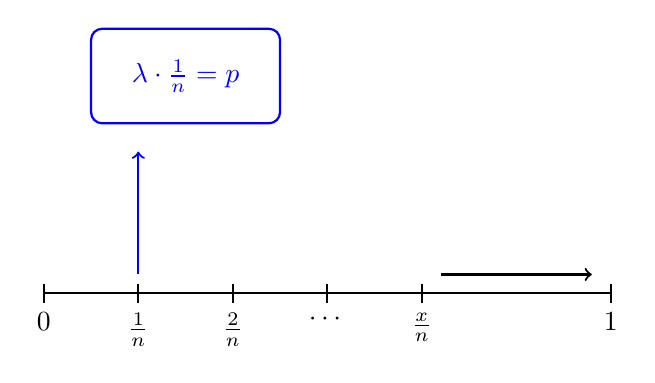
\begin{tikzpicture}[scale=1.2]
  % Línea horizontal del intervalo [0,1]
  \draw[thick] (0,0) -- (6,0);
  
  % Marcas de división
  \draw[thick] (0,0.1) -- (0,-0.1) node[below] {$0$};
  \draw[thick] (1,0.1) -- (1,-0.1) node[below] {$\frac{1}{n}$};
  \draw[thick] (2,0.1) -- (2,-0.1) node[below] {$\frac{2}{n}$};
  \draw[thick] (3,0.1) -- (3,-0.1) node[below] {$\cdots$};
  \draw[thick] (4,0.1) -- (4,-0.1) node[below] {$\frac{x}{n}$};
  \draw[thick] (6,0.1) -- (6,-0.1) node[below] {$1$};
  
  % Flecha desde 1/n hacia abajo
  \draw[->, thick, blue] (1,0.2) -- (1,1.5);
  
  % Caja con la ecuación λ⋅1/n = P
  \draw[thick, blue, rounded corners] (0.5,1.8) rectangle (2.5,2.8);
  \node[blue] at (1.5,2.3) {$\lambda \cdot \frac{1}{n} = p$};
  
  % Flecha desde x/n hacia la derecha
  \draw[->, thick] (4.2,0.2) -- (5.8,0.2);
\end{tikzpicture}
\end{center}

\begin{equation*}
P(X = x) = \text{Bin}(n, p = \tfrac{\lambda}{n})
\end{equation*}

\teorema{Si $X_n \sim \text{Bin}(n, p(n))$ y $n \, p(n) \to \lambda$ cuando $n \to \infty$, entonces
\begin{equation*}
X_n \xrightarrow{d} \text{Poisson}(\lambda)
\end{equation*}}

\teorema{Las definiciones (1) y (2) son equivalentes:
\begin{itemize}
    \item $N(0) = 0$
    \item Incrementos estacionarios e independientes; los incrementos tienen distribución Poisson
\end{itemize}}

\textbf{Demostración:}

empezamos por demostrar que (2) $= >$ (1)

\begin{equation*}
P_n(t) = P(N(t) = n) \quad \longleftarrow \quad \text{distribución Poisson}(\lambda t)
\end{equation*}

\begin{equation*}
P'_n(t) = \lim_{\varepsilon \to 0} \frac{P_n(t+\varepsilon) - P_n(t)}{\varepsilon}
\end{equation*}

\begin{equation*}
\frac{P_n(t+\varepsilon) - P_n(t)}{\varepsilon}
= \frac{P(N(t+\varepsilon)=n) - P(N(t)=n)}{\varepsilon}\; ?
\end{equation*}

\begin{align*}
P(N(t+\varepsilon) = n) 
&= P(N(t)=n,\; N(t+\varepsilon)-N(t)=0) \\
&\quad + P(N(t)=n-1,\; N(t+\varepsilon)-N(t)=1) \\
&\quad + P(N(t)\leq n-2,\; N(t+\varepsilon)-N(t)\geq 2) \\
&= P(N(t)=n)\cdot P(N(t+\varepsilon)-N(t)=0) \\
&\quad + P(N(t)=n-1)\cdot P(N(t+\varepsilon)-N(t)=1) \\
&\quad + P(N(t)\leq n-2)\cdot P(N(t+\varepsilon)-N(t)\geq 2) \\
&= P_n(t)P_0(\varepsilon) + P_{n-1}(t)P_1(\varepsilon) + o(\varepsilon).
\end{align*}


\begin{align*}
P_0(\varepsilon) &= P(N(\varepsilon)=0) 
= 1 - P(N(\varepsilon)\geq 1) \\
&= 1 - P(N(\varepsilon)=1) - P(N(\varepsilon)\geq 2) \\
&= 1 - \lambda \varepsilon + o(\varepsilon) + o(\varepsilon) \\
&= 1 - \lambda \varepsilon + o(\varepsilon)
\end{align*}

\begin{align*}
P_1(\varepsilon) &= P(N(\varepsilon)=1) \\
&= \lambda \varepsilon + o(\varepsilon)
\end{align*}

\begin{align*}
P_n(t+\varepsilon) 
&= P_n(t)\,(1 - \lambda \varepsilon + o(\varepsilon)) 
   + P_{n-1}(t)\,(\lambda \varepsilon + o(\varepsilon)) 
   + o(\varepsilon) \\
&= P_n(t) - \lambda \varepsilon P_n(t) + o(\varepsilon)P_n(t) \\
&\quad + \lambda \varepsilon P_{n-1}(t) + o(\varepsilon)P_{n-1}(t) 
   + o(\varepsilon)
\end{align*}

\begin{align*}
P_n(t+\varepsilon) &= P_n(t) + \lambda \varepsilon (P_{n-1}(t) - P_n(t)) + o(\varepsilon)
\end{align*}

Así:

\begin{align*}
\frac{P_n(t+\varepsilon) - P_n(t)}{\varepsilon} 
&= \frac{P_n(t) + \lambda \varepsilon (P_{n-1}(t) - P_n(t)) + o(\varepsilon) - P_n(t)}{\varepsilon} \\
&= \lambda (P_{n-1}(t) - P_n(t)) + \frac{o(\varepsilon)}{\varepsilon}
\end{align*}

Tomando el límite cuando $\varepsilon \to 0$:

\begin{align*}
P'_n(t) &= \lambda (P_{n-1}(t) - P_n(t))
\end{align*}

\begin{align*}
P_n'(t) + \lambda P_n(t) &= \lambda P_{n-1}(t) \\
e^{\lambda t} P_n'(t) + e^{\lambda t} \lambda P_n(t) &= e^{\lambda t} \lambda P_{n-1}(t) \\
\left(e^{\lambda t} P_n(t)\right)' &= \lambda e^{\lambda t} P_{n-1}(t)
\end{align*}

\textbf{Inducción en $n$}:

Para $n=1$:

\begin{align*}
\left(e^{\lambda t} P_1(t)\right)' &= \lambda e^{\lambda t} P_0(t) \\
                                   &= \lambda e^{\lambda t} e^{-\lambda t} \\
                                   &= \lambda
\end{align*}

\begin{align*}
P_0(t) &= e^{-\lambda t} \\
\left(e^{\lambda t} P_1(t)\right)' &= \lambda \\
e^{\lambda t} P_1(t) - e^{\lambda \cdot 0} P_1(0) &= \lambda t \\
e^{\lambda t} P_1(t) &= \lambda t \\
P_1(t) &= e^{-\lambda t} \lambda t
\end{align*}

\textbf{Hipótesis de inducción:}
\begin{align*}
P_{n-1}(t) = e^{-\lambda t} \frac{(\lambda t)^{n-1}}{(n-1)!}
\end{align*}

\textbf{Por demostrar:}
\begin{align*}
P_n(t) = e^{-\lambda t} \frac{(\lambda t)^n}{n!}
\end{align*}

Ahora se va a demostrar que (1) $= >$ (2)

Si $N(t) \sim \text{Poisson}(\lambda t)$ entonces:

\begin{enumerate}
    \item $P(N(h)=1) = e^{-\lambda h} \lambda h$
    \item $P(N(h) \geq 2) = o(h)$
\end{enumerate}

\textbf{Demostración de 1)}:

\begin{align*}
P(N(h)=1) &= e^{-\lambda h} \lambda h \\
&= (1 - \lambda h + o(h)) \lambda h \\
&= \lambda h - \lambda^2 h^2 + o(h) \lambda h \\
&= \lambda h + o(h)
\end{align*}

\textbf{Demostración de 2)}:

\begin{align*}
P(N(h) \geq 2) &= 1 - P(N(h)=0) - P(N(h)=1) \\
&= 1 - e^{-\lambda h} - e^{-\lambda h} \lambda h \\
&= 1 - (1 - \lambda h + o(h)) - (\lambda h + o(h)) \\
&= 1 - 1 + \lambda h - o(h) - \lambda h - o(h) \\
&= o(h)
\end{align*}

Por lo tanto, se ha demostrado que las definiciones (1) y (2) son equivalentes.

% Continuacion de la clase 02 septiembre 01 2025
% ===================== Contenido del pizarrón =====================

\textbf{Proceso de Poisson}

\definicion{
(1) Un proceso de Poisson cumple:
\begin{enumerate}
    \item $N(0) = 0$
    \item Tiene incrementos independientes
    \item Tiene incrementos estacionarios
    \begin{equation*}
    N(t+s) - N(s) \sim \text{Poisson}(\lambda s)
    \end{equation*}
\end{enumerate}
}

\definicion{(2) Se dice que un proceso de conteo $\{N(t)\}_{t \geq 0}$ es un \textbf{proceso de Poisson} con tasa $\lambda > 0$, si cumple:
\begin{enumerate}
    \item $N(0) = 0$,
    \item El proceso tiene incrementos estacionarios e independientes,
    \item $P(N(h) = 1) = \lambda h + o(h)$,
    \item $P(N(h) \geq 2) = o(h)$.
\end{enumerate}}

\definicion{(3) Sean $t_1, t_2, t_3, (iid) \sim \text{exp}(\lambda)$. Y sea $T_n = \sum_{i=1}^{n} t_i$ con $T_0 = 0$, el proceso $N(s) = \max\{n : T_n \leq s\}$ es un proceso de Poisson.}


\lema{$N(s)$ tiene distribución Poisson$(\lambda s)$.}

\textbf{Idea de la demostración:}

Nota: $\int_0^{\infty} \lambda (\lambda x)^{n-1} \frac{e^{-\lambda x}}{(n-1)!} dx = 1 - \sum_{k=0}^{n-1} \frac{(\lambda t)^k}{k!} e^{-\lambda t}$

\begin{equation*}
\{N(t) < n\} \Leftrightarrow \{T_n \geq t\}
\end{equation*}
\begin{equation*}
P(N(t) < n) = P(T_n \geq t), \quad T_n \sim \text{Gamma}(n, \lambda)
\end{equation*}

\begin{equation*}
= \int_t^{\infty} \frac{\lambda (\lambda x)^{n-1} e^{-\lambda x}}{(n-1)!} dx = 1 - \int_0^t \frac{\lambda (\lambda x)^{n-1} e^{-\lambda x}}{(n-1)!} dx
\end{equation*}

\begin{equation*}
= 1 - 1 + \sum_{k=0}^{n-1} \frac{(\lambda t)^k}{k!} e^{-\lambda t}
\end{equation*}

\begin{equation*}
= \sum_{k=0}^{n-1} \frac{(\lambda t)^k}{k!} e^{-\lambda t}
\end{equation*}

Tarea:
\begin{equation*}
P(N(t) = n) = \sum_{k=0}^{n} \frac{(\lambda t)^k}{k!} e^{-\lambda t} - \sum_{k=0}^{n-1} \frac{(\lambda t)^k}{k!} e^{-\lambda t}
\end{equation*}

\begin{equation*}
\Rightarrow N(t) \sim \text{Poisson}(\lambda t).
\end{equation*}

\lema{$N(t+c) - N(c)$, $t \geq 0$ es un proceso de Poisson con tasa $\lambda$ e independiente de $N(r)$; $0 \leq r \leq s$.}

\textbf{Idea de la demostración}

\begin{center}
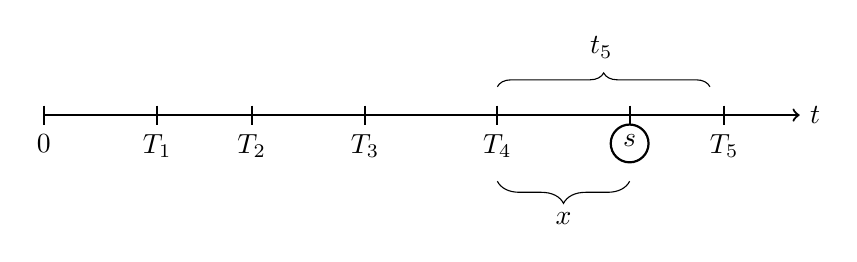
\begin{tikzpicture}[scale=1.2]
  % Línea temporal principal
  \draw[thick,->] (0,0) -- (8,0) node[right] {$t$};
  
  % Marcas de tiempo con líneas verticales
  \draw[thick] (0,0.1) -- (0,-0.1) node[below] {$0$};
  \draw[thick] (1.2,0.1) -- (1.2,-0.1) node[below] {$T_1$};
  \draw[thick] (2.2,0.1) -- (2.2,-0.1) node[below] {$T_2$};
  \draw[thick] (3.4,0.1) -- (3.4,-0.1) node[below] {$T_3$};
  \draw[thick] (4.8,0.1) -- (4.8,-0.1) node[below] {$T_4$};
  
  % Marca especial para s con círculo
  \draw[thick] (6.2,0.1) -- (6.2,-0.1);
  \draw[thick] (6.2,-0.3) circle (0.2);
  \node[below] at (6.2,-0.1) {$s$};
  
  % T_5 después de s
  \draw[thick] (7.2,0.1) -- (7.2,-0.1) node[below] {$T_5$};
  
  \draw[decorate,decoration={brace,amplitude=5pt}] (4.8,0.3) -- (7.05,0.3);
  \node[above] at (5.9,0.5) {$t_5$};

  % Llave inferior desde T_4 hasta s
  \draw[decorate,decoration={brace,amplitude=8pt,mirror}] (4.8,-0.7) -- (6.2,-0.7);
  \node at (5.5,-1.1) {$x$};
  
\end{tikzpicture}
\end{center}

\begin{equation*}
P(t_5 > x+t \mid t_5 > x) = P(t_5 > t) = \exp(\lambda)
\end{equation*}

\textbf{Tarea: Definición (1) $\longleftrightarrow$ Definición (3)}

\subsection{Características de un Proceso de Poisson}

\teorema{Sea $\{N(t)\}_{t \geq 0}$ un proceso de Poisson $(\lambda)$. Suponga que para un $t > 0$ fijo, $N(t) = n$. Entonces para $0 \leq u < t$, el número de eventos que han ocurrido antes de $u$ es una v.a. Bin$(n, \frac{u}{t})$, es decir:
\begin{equation*}
P(N(u) = x \mid N(t) = n) = \binom{n}{x} \left(\frac{u}{t}\right)^x \left(1 - \frac{u}{t}\right)^{n-x}
\end{equation*}}

\begin{center}
\begin{tikzpicture}[scale=1.2]
  % Línea temporal
  \draw[thick] (0,0) -- (6,0);
  \draw (0,0) node[below] {$0$} -- +(0,0.2);
  \draw (3,0) node[below] {$u$} -- +(0,0.2);
  \draw (6,0) node[below] {$t$} -- +(0,0.2);
  
  % Llaves
  % Llave superior para n (cubre todo de 0 a t)
  \draw[decorate,decoration={brace,amplitude=10pt}] (0,0.5) -- (6,0.5);
  \node at (3,1) {$n$};
  
  % Llave inferior para x (cubre de 0 a u)
  \draw[decorate,decoration={brace,amplitude=10pt,mirror}] (0,-0.5) -- (3,-0.5);
  \node at (1.5,-1) {$x$};
\end{tikzpicture}
\end{center}

\textbf{Demostración:}

\begin{align*}
P(N(u) = x \mid N(t) = n) &= \frac{P(N(u) = x, N(t) = n)}{P(N(t) = n)} \\
&= \frac{P(N(u) = x, N(t) - N(u) = n - x)}{P(N(t) = n)}
\end{align*}

Por independencia de incrementos:

\begin{equation*}
= \frac{P(N(u) = x) \cdot P(N(t) - N(u) = n - x)}{P(N(t) = n)}
\end{equation*}

\begin{equation*}
= \frac{\frac{e^{-\lambda u} (\lambda u)^x}{x!} \cdot \frac{e^{-\lambda(t-u)} (\lambda(t-u))^{n-x}}{(n-x)!}}{\frac{e^{-\lambda t} (\lambda t)^n}{n!}}
\end{equation*}

\begin{equation*}
= \frac{n!}{x!(n-x)!} \cdot \frac{(\lambda u)^x (\lambda(t-u))^{n-x}}{(\lambda t)^n (\lambda t)^{n-x}}
\end{equation*}

\begin{equation*}
= \binom{n}{x} \frac{(\lambda u)^x (\lambda(t-u))^{n-x}}{(\lambda t)^x (\lambda t)^{n-x}}
\end{equation*}

\begin{equation*}
= \binom{n}{x} \left(\frac{\lambda u}{\lambda t}\right)^x \left(\frac{\lambda(t-u)}{\lambda t}\right)^{n-x}
\end{equation*}

\begin{equation*}
= \binom{n}{x} \left(\frac{u}{t}\right)^x \left(\frac{t-u}{t}\right)^{n-x}
\end{equation*}

\begin{equation*}
= \binom{n}{x} \left(\frac{u}{t}\right)^x \left(1 - \frac{u}{t}\right)^{n-x}
\end{equation*}

\teorema{Sean $N_1, N_2, \ldots, N_k$ procesos de Poisson independientes con intensidades $\lambda_1, \lambda_2, \ldots, \lambda_k$ entonces:
\begin{equation*}
N = N_1 + N_2 + \cdots + N_k
\end{equation*}
es un proceso de Poisson con tasa $\lambda_1 + \lambda_2 + \cdots + \lambda_k$.}

\textbf{Demostración}: $k = 2$

\begin{itemize}
    \item $N(0) = 0$
    
    Porque: $N_1(0) = 0$, $N_2(0) = 0$
    
    \item $t_1 < t_2 < t_3$
    
    $* N_1(t_3) - N_1(t_2)$ ind $N_1(t_2) - N_1(t_1)$
    
    $* N_2(t_3) - N_2(t_2)$ ind $N_2(t_2) - N_2(t_1)$
    
    $N(t_3) - N(t_2) = N_1(t_3) + N_2(t_3) - N_1(t_2) - N_2(t_2)$
    
    $= N_1(t_3) - N_1(t_2) + N_2(t_3) - N_2(t_2)$
    
    es independiente de
    
    $N_1(t_2) - N_1(t_1) + N_2(t_2) - N_2(t_1)$
    
    $= N(t_2) - N(t_1)$.
    
    \item $N(t+s) - N(s) = N_1(t+s) + N_2(t+s) - N_1(s) - N_2(s)$
    
    $= N_1(t+s) - N_1(s) + N_2(t+s) - N_2(s)$
    
    $\sim \text{Poisson}(\lambda_1 t)$ ind $\text{Poisson}(\lambda_2 t)$
    
    $\sim \text{Poisson}((\lambda_1 + \lambda_2)t)$.
\end{itemize}

\begin{equation*}
= \frac{P(N(u) = x) \cdot P(N(t) - N(u) = n - x)}{\frac{e^{-\lambda t} (\lambda t)^n}{n!}}
\end{equation*}

\begin{equation*}
= \frac{\frac{e^{-\lambda u} (\lambda u)^x}{x!} \cdot \frac{e^{-\lambda(t-u)} (\lambda(t-u))^{n-x}}{(n-x)!}}{\frac{e^{-\lambda t} (\lambda t)^n}{n!}}
\end{equation*}

\begin{equation*}
= \frac{n!}{x!(n-x)!} \cdot \frac{(\lambda u)^x (\lambda(t-u))^{n-x}}{(\lambda t)^x (\lambda t)^{n-x}}
\end{equation*}

\begin{equation*}
= \binom{n}{x} \left(\frac{\lambda u}{\lambda t}\right)^x \left(\frac{\lambda(t-u)}{\lambda t}\right)^{n-x}
\end{equation*}

\teorema{Sea $N$ un proceso de Poisson $(\lambda)$ y $N_j$ número de eventos de tipo $j$ tal que $P(\text{tipo } j) = P_j$, $j = 1, \ldots, k$, entonces $N_j$ es un proceso de Poisson$(\lambda P_j)$.}

\textbf{Demostración}: $k = 2$.

$P(\text{tipo } 1) = p$, $P(\text{tipo } 2) = 1 - p$.

1) $N_1(0) = 0$, $N_2(0) = 0$.

2) $N_1$ y $N_2$ tienen incrementos independientes y estacionarios, por que $N$ los tiene.

3) Sea $X_1 = N_1(t+s) - N_1(s)$

$X_2 = N_2(t+s) - N_2(s)$.

$P(X_1 = n, X_2 = k) =$

$= P(X_1 = n, X_2 = k) \cdot \frac{P(X_1 + X_2 = n+k)}{P(X_1 + X_2 = n+k)}$

$= P(X_1 = n, X_2 = k \mid X_1 + X_2 = n+k) P(X_1 + X_2 = n+k)$.

$= P(X_1 = n, X_2 = k \mid X_1 + X_2 = n+k) P(X_1 + X_2 = n+k)$.

$= \frac{e^{-\lambda t} (\lambda t)^{n+k}}{(n+k)!} \binom{n+k}{n} p^n (1-p)^k$

\begin{center}
\fbox{\begin{minipage}{0.8\textwidth}
\begin{equation*}
\frac{P(\overbrace{(X_1 = n, X_2 = k)}^{A}, \overbrace{X_1 + X_2 = n+k}^{B})}{P(X_1 + X_2 = n+k)}
\end{equation*}

$A \subseteq B$

$A \cap B = A$

\begin{equation*}
= \frac{P(X_1 = n, X_2 = k)}{P(X_1 + X_2 = n+k)}.
\end{equation*}
\end{minipage}}
\end{center}

$= e^{-\lambda t p} e^{-\lambda t(1-p)} (\lambda t)^n (\lambda t)^k p^n (1-p)^k \frac{(n+k)!}{n! \cdot k!}$

$= e^{-\lambda t p} \frac{(\lambda t p)^n}{n!} e^{-\lambda t(1-p)} \frac{(\lambda t(1-p))^k}{k!}$

$= \text{Poisson}(\lambda t p) \cdot \text{Poisson}(\lambda t(1-p))$

$P(X_1 = n, X_2 = k) = \text{Poisson}(\lambda t p) \cdot P(\lambda t(1-p))$

\vspace{1cm}

\begin{center}
\begin{tikzpicture}[scale=1.2]
  % Línea temporal
  \draw[thick] (0,0) -- (6,0);
  \draw (0,0) node[below] {$0$} -- +(0,0.2);
  \draw (3,0) node[below] {$u$} -- +(0,0.2);
  \draw (6,0) node[below] {$t$} -- +(0,0.2);
  
  % Llaves
  % Llave superior para n (cubre todo de 0 a t)
  \draw[decorate,decoration={brace,amplitude=10pt}] (0,0.5) -- (6,0.5);
  \node at (3,1) {$n$};
  
  % Llave inferior para x (cubre de 0 a u)
  \draw[decorate,decoration={brace,amplitude=10pt,mirror}] (0,-0.5) -- (3,-0.5);
  \node at (1.5,-1) {$x$};
\end{tikzpicture}
\end{center}

Bin$(n, \frac{u}{t})$

\teorema{Sea $N(t)$ un proceso de Poisson con tasa $\lambda$, y suponga que para $t > 0$ fijo, se sabe que $N(t) = n$. Entonces $T_1, T_2, \ldots, T_n$ dado $N(t) = n$ tiene densidad
\begin{equation*}
f(t_1, t_2, \ldots, t_n \mid N(t) = n) = \frac{n!}{t^n}, \quad 0 < t_1 < t_2 < \ldots < t_n
\end{equation*}}

\textbf{Demostración}: $0 < t_1 < t_2 < t_3 < \ldots < t_n < t$.

\begin{equation*}
F(t_1, \ldots, t_n \mid N(t) = n) = P(T_1 \leq t_1, T_2 \leq t_2, \ldots, T_n \leq t_n \mid N(t) = n)
\end{equation*}

\begin{equation*}
= \frac{P(T_1 \leq t_1, \ldots, T_n \leq t_n, N(t) = n)}{P(N(t) = n)}
\end{equation*}

Nota que: $\{T_1 \leq t_1, \ldots, T_n \leq t_n, N(t) = n\}$ es equivalente al evento "un y solo un cliente llega en los intervalos $[0, t_1], [t_1, t_2], \ldots, [t_{n-1}, t_n]$ y ningún cliente llega en $(t_n, t]$.

\begin{equation*}
P(t_1, \ldots, t_n \mid n) = \frac{e^{-\lambda t_1} \lambda t_1 \cdot e^{-\lambda(t_2-t_1)} \lambda(t_2-t_1) \cdots e^{-\lambda(t_n-t_{n-1})} \lambda(t_n-t_{n-1}) e^{-\lambda(t-t_n)}}{\frac{e^{-\lambda t} (\lambda t)^n}{n!}}
\end{equation*}

\begin{equation*}
= \frac{e^{-\lambda t} \lambda^n (t_1(t_2-t_1)\cdots(t_n-t_{n-1}))}{\frac{e^{-\lambda t} \lambda^n t^n}{n!}}
\end{equation*}

\begin{equation*}
= \frac{n! (t_1(t_2-t_1)\cdots(t_n-t_{n-1}))}{t^n}
\end{equation*}

Tarea:
\begin{equation*}
\frac{\partial^n F}{\partial t_1 \partial t_2 \cdots \partial t_n} = \frac{n!}{t^n}
\end{equation*}

% el profesor aca menciona algo sobre la base de datos


%% fin de la clase 02 septiembre 01 2025

%% Clase 8 de septiembre

\section{Proceso de Poisson compuesto}

Sea $X_1, X_2, \ldots$ i.i.d., $N$ variable aleatoria entera no negativa.

\begin{equation*}
  S_N = \sum_{i=1}^{N} X_i, \quad S_t = \sum_{i=1}^{0} X_i
\end{equation*}

\begin{align*}
E(S_N) &= \sum_{i=1}^{N} E(X_i) = N E(X_i), \\
\mathrm{Var}(S_N) &= N\, \mathrm{Var}(X_i), \\
E(X|Y=y) &= \sum_{x} x\, P(X=x|Y=y), \\
E(Y) &= \sum_{y} y\, P(y)
\end{align*}


\teorema{(Esperanza total) Para variables aleatorias $X$ e $Y$,
\begin{equation*}
E(X) = E_Y\big(E(X|Y)\big)
\end{equation*}
}

\textbf{Demostración:}

\begin{align*}
E_Y(E(X|Y)) &= E\left(\sum_x x \cdot P(X=x|Y)\right) \\
&= \sum_y \sum_x x \cdot P(X=x|Y=y) P(Y=y) \\
&= \sum_y \sum_x x \cdot \frac{P(X=x, Y=y)}{P(Y=y)} P(Y=y) \\
&= \sum_y \sum_x x \cdot P(X=x, Y=y) \\
&= \sum_x x \sum_y P(X=x, Y=y) \\
&= \sum_x x \cdot P(X=x) \\
&= E(X)
\end{align*}

\teorema{Sean $X_1, X_2, \ldots$ i.i.d. con primer y segundo momento finito. Sea $N$ una v.a. independiente y discreta. Consideremos $S_N = \sum_{i=1}^{N} X_i$ con $S_0 = 0$.
\begin{enumerate}
\item Si $E(N) < \infty$ entonces $E(S_N) = E(N) \cdot E(X_1)$
\item Si $E(N^2) < \infty$ entonces $\text{Var}(S_N) = E(N) \text{Var}(X_1) + \text{Var}(N) [E(X_1)]^2$
\end{enumerate}}

\textbf{Demostración:}

1) $E(S_N) = E_N(E(S_N|N))$

\begin{align*}
&= \sum_n E(S_n|N=n) P(N=n) \\
&= \sum_n E(S_n|N=n) \cdot P(N=n) \\
&= \sum_n E(S_n) \cdot P(N=n) \\
&= \sum_n n E(X_1) \cdot P(N=n) \\
&= E(X_1) \sum_n n P(N=n) \\
&= E(N) \cdot E(X_1)
\end{align*}

2) $\text{Var}(S_N) = E(S_N^2) - [E(S_N)]^2$

Calculamos $E(S_N^2)$:

\begin{align*}
E(S_N^2) &= E_N(E(S_N^2|N)) \\
&= \sum_n E(S_n^2|N=n) P(N=n) \\
&= \sum_n E(S_n^2) P(N=n)
\end{align*}

Donde:
\begin{align*}
\text{Var}(S_n) &= E(S_n^2) - [E(S_n)]^2 \\
n\text{Var}(X_1) &= E(S_n^2) - n^2[E(X_1)]^2 \\
E(S_n^2) &= n\text{Var}(X_1) + n^2[E(X_1)]^2
\end{align*}

Entonces:
\begin{align*}
E(S_N^2) &= \sum_n \left(n\text{Var}(X_1) + n^2[E(X_1)]^2\right) P(N=n) \\
&= \text{Var}(X_1) \sum_n n P(N=n) + [E(X_1)]^2 \sum_n n^2 P(N=n) \\
&= E(N)\text{Var}(X_1) + [E(X_1)]^2 E(N^2)
\end{align*}

Finalmente:
\begin{align*}
\text{Var}(S_N) &= E(N)\text{Var}(X_1) + [E(X_1)]^2 E(N^2) - [E(N)]^2[E(X_1)]^2 \\
&= E(N)\text{Var}(X_1) + [E(X_1)]^2\left(E(N^2) - [E(N)]^2\right) \\
&= E(N)\text{Var}(X_1) + [E(X_1)]^2\text{Var}(N)
\end{align*}

\textbf{Observación}: Sea $N(t)$ un proceso de Poisson($\lambda$), entonces definimos 
\begin{equation*}
S_t = \sum_{i=1}^{N(t)} X_i
\end{equation*}
que es llamado un proceso de Poisson compuesto.

\begin{align*}
E(S_t) &= E(N(t)) E(X_1) \\
&= \lambda t E(X_1)
\end{align*}

\begin{align*}
\text{Var}(S_t) &= E(N(t))\text{Var}(X_1) + [E(X_1)]^2\text{Var}(N(t)) \\
&= \lambda t \text{Var}(X_1) + \lambda t [E(X_1)]^2 \\
&= \lambda t \left(\text{Var}(X_1) + [E(X_1)]^2\right) \\
&= \lambda t E(Y_1^2)
\end{align*}

\textbf{Problema:} Un pescador captura truchas siguiendo un proceso de Poisson con una intensidad de 3 pescados por hora. Supongamos que las truchas pesan un promedio de 4 libras con una desviación estándar de 2 libras.

Determinar la media y varianza del peso total de los peces que captura en 2 horas.

\textbf{Solución:}

\begin{itemize}
    \item $N(t)$ : Número de truchas que salen hasta el tiempo $t$.
    \item $X_i$ : El peso de la trucha $i$-ésima.
    \item $S_t = \sum_{i=1}^{N(t)} X_i$ : Peso total de las truchas sacadas hasta el tiempo $t$ (horas).
\end{itemize}

\begin{align*}
E(S_2) &= E(N(2)) \cdot E(X_1) \\
&= 6 \times 4 = 24 \text{ libras}
\end{align*}

\begin{align*}
\text{Var}(S_t) &= \lambda t E(X_1^2) = \lambda t \left(\text{Var}(X_1) + [E(X_1)]^2\right) \\
&= 6(4 + 16) = 120 \text{ libras}^2
\end{align*}

\section{Cadenas de Markov en tiempo continuo}

\definicion{Un proceso en tiempo continuo $\{X_t\}_{t \geq 0}$ es una \textbf{cadena de Markov} si, 
para cualquier $0 \leq s_0 \leq s_1 \leq \cdots \leq s_n \leq s$ y para cualquier conjunto de estados $i_0, i_1, \dots, i_n, i, j$ se cumple:
\begin{equation*}
\mathbb{P}\bigl(X_{t+s} = j \,\big|\, X_s = i,\, X_{s_n} = i_n,\, \dots,\, X_{s_0} = i_0 \bigr)
= 
\mathbb{P}\bigl(X_{t+s} = j \,\big|\, X_s = i \bigr).
\end{equation*}}

\textbf{Ejemplo}: (Transformación de una cadena de Markov a tiempo continuo) Sea $N(t)$ un proceso de Poisson con intensidad $\lambda$ y sea $Y_n$ una cadena de Markov con matriz de transición $U(i,j)$, $i \neq j$. Entonces $X_t = Y_{N(t)}$ es una cadena de Markov en tiempo continuo.

\begin{center}
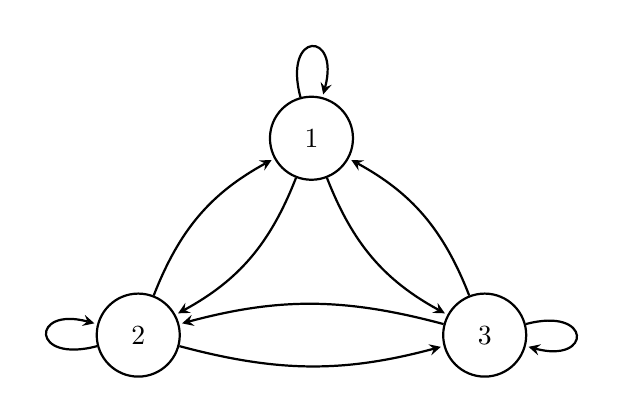
\begin{tikzpicture}[->,>=stealth,shorten >=1pt,auto,node distance=3cm,semithick]
\tikzstyle{every state}=[fill=white,draw=black,text=black,minimum size=30pt,thick]

% Posicionar nodos en triángulo equilátero
\node[state] (1) at (0,2.5) {$1$};
\node[state] (2) at (-2.2,0) {$2$};
\node[state] (3) at (2.2,0) {$3$};

% Bucles en cada estado
\path[thick]
(1) edge[loop above] node{} (1)
(2) edge[loop left] node{} (2)
(3) edge[loop right] node{} (3);

% Conexiones entre estados
\path[thick]
% De 1 a 2 y viceversa
(1) edge[bend left=20] node{} (2)
(2) edge[bend left=20] node{} (1)
% De 1 a 3 y viceversa
(1) edge[bend right=20] node{} (3)
(3) edge[bend right=20] node{} (1)
% De 2 a 3 y viceversa
(2) edge[bend right=15, below] node{} (3)
(3) edge[bend right=15, above] node{} (2);
\end{tikzpicture}
\end{center}

\begin{center}
\begin{tikzpicture}
\draw[->] (0,0) -- (8,0);
\node[below] at (0,0) {0};
\node[below] at (2,0) {$x$};
\node[below] at (4,0) {$x$};
\node[above] at (0,0) {$N(t)$};
\end{tikzpicture}
\end{center}

\definicion{Para $t > 0$ la probabilidad de transición es definida por:
\begin{equation*}
P_t(i,j) = P(X_t = j | X_0 = i)
\end{equation*}}

\textbf{Problema:} Calcule la probabilidad de transición del proceso $X_t = Y_{N(t)}$.

\textbf{Solución:}

\begin{align*}
P_t(i,j) &= P(X_t = j | X_0 = i) \\
&= P\left(Y_{N(t)} = j \mid Y_0 = i\right) \\
&= \sum_{n=1}^{\infty} P\left(Y_{N(t)} = j, N(t) = n \mid Y_0 = i\right) \\
&= \sum_{n=0}^{\infty} P\left(Y_n = j \mid Y_0 = i\right) P(N(t) = n) \\
&= \sum_{n=0}^{\infty} U^n(i,j) \frac{e^{-\lambda t}(\lambda t)^n}{n!}
\end{align*}

\definicion{La tasa de saltos de una cadena de Markov con probabilidades de transición $P_t(i,j)$ está dada por:
\begin{equation*}
q(i,j) = \lim_{\varepsilon \to 0} \frac{P_\varepsilon(i,j)}{\varepsilon}
\end{equation*}
para $i \neq j$.}

\textbf{Problema:} Tasa de saltos de un proceso de Poisson

Nota que:

\begin{itemize}
    \item $P_\varepsilon(i,j) = 0$ para $j < i$
    \item $P_\varepsilon(i,j) = P(N(\varepsilon) > 1)$ para $j > i+1$\\
    \hspace{1.5em} $= O(\varepsilon)$
    \item $P_\varepsilon(i, i+1) = P(N(\varepsilon) = 1)$\\
    \hspace{1.5em} $= \lambda\varepsilon + O(\varepsilon)$
\end{itemize}

Si $j \neq i$:
\begin{equation*}
q(i,j) = \lim_{\varepsilon \to 0} \frac{P_\varepsilon(i,j)}{\varepsilon} = 0
\end{equation*}

Si $j > i+1$:
\begin{equation*}
q(i,j) = \lim_{\varepsilon \to 0} \frac{P_\varepsilon(i,j)}{\varepsilon} = \lim_{\varepsilon \to 0} \frac{O(\varepsilon)}{\varepsilon} = 0
\end{equation*}

Si $j = i+1$:
\begin{equation*}
q(i,j) = \lim_{\varepsilon \to 0} \frac{P_\varepsilon(i,j)}{\varepsilon} = \lim_{\varepsilon \to 0} \frac{\lambda\varepsilon + O(\varepsilon)}{\varepsilon} = \lambda
\end{equation*}

Por lo tanto:
\begin{equation*}
q(i,j) = \begin{cases}
0 & \text{si } j \neq i+1 \\
\lambda & \text{si } j = i+1
\end{cases}
\end{equation*}

\textbf{Problema:} Tasa de saltos del proceso $Y_{N(t)} = X_t$

\begin{equation*}
P_\varepsilon(i,j) = \sum_{n=1}^{\infty} \frac{e^{-\lambda\varepsilon}(\lambda\varepsilon)^n}{n!} U^n(i,j)
\end{equation*}

¿Cuál es $q(i,j)$, $i \neq j$?

\begin{equation*}
\frac{P_\varepsilon(i,j)}{\varepsilon} = \frac{e^{-\lambda\varepsilon} \lambda\varepsilon U(i,j)}{\varepsilon} + \sum_{n=2}^{\infty} \frac{e^{-\lambda\varepsilon}(\lambda\varepsilon)^n}{n!} \frac{U^n(i,j)}{\varepsilon}
\end{equation*}

\begin{equation*}
\xrightarrow{\varepsilon \to 0} \lambda U(i,j)
\end{equation*}

\begin{equation*}
q(i,j) = \begin{cases}
\lambda U(i,j) & \text{si } i \neq j \\
0 & \text{e.o.c.}
\end{cases}
\end{equation*}

\begin{center}
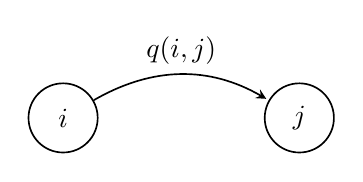
\begin{tikzpicture}[->,>=stealth,shorten >=1pt,auto,node distance=3cm,semithick]
\tikzstyle{every state}=[fill=white,draw=black,text=black,minimum size=25pt]
\node[state] (i) {$i$};
\node[state] (j) [right of=i] {$j$};
\path (i) edge[bend left] node[above] {$q(i,j)$} (j);
\end{tikzpicture}
\end{center}

% ===================== Tasas de salida =====================

\textbf{Si tenemos las tasas, ¿cómo reconstruimos la cadena?}

\begin{equation*}
\lambda_i = \sum_{j \neq i} q(i,j)
\end{equation*}

\begin{enumerate}
    \item $\lambda_i = \infty$; no se puede entrar al $i$.
    \item $\lambda_i = 0$; $i$ es absorbente.
    \item $0 < \lambda_i < \infty$.
\end{enumerate}

La probabilidad de saltar del estado $i$ al estado $j$ es:

\begin{equation*}
r(i,j) = \frac{q(i,j)}{\lambda_i}
\end{equation*}

% ===================== Simulación =====================

\textbf{Simulación}: $X_t$ una cadena de Markov en tiempo continuo. $q(i,j)$ las tasas de salto de la cadena y $0 < \lambda_i < \infty$ para todo $i \in S$.

\begin{itemize}
    \item Se mantiene en el estado $i$ un tiempo $\exp(\lambda_i)$.
    \item Después salta a un estado $j$ con probabilidad $r(i,j)$.
\end{itemize}

\textbf{Ejemplo}: Simulación de un Proceso de Poisson.

\begin{equation*}
\lambda_i = \sum_{j \neq i} q(i,j) = q(i,i+1) = \lambda
\end{equation*}

\begin{equation*}
r(i,j) = \frac{q(i,j)}{\lambda_i} = \begin{cases}
0 & \text{si } j \neq i+1 \\
\frac{\lambda}{\lambda} = 1 & \text{si } j = i+1
\end{cases}
\end{equation*}

\textbf{Ejemplo}: Simulación $X_t = Y_{N(t)}$.

\begin{equation*}
q(i,j) = \begin{cases}
\lambda U(i,j) & \text{para } i \neq j \\
0 & \text{e.o.c.}
\end{cases}
\end{equation*}

\begin{equation*}
\lambda_i = \sum_{j \neq i} q(i,j) = \lambda \sum_{j \neq i} U(i,j) = \lambda
\end{equation*}

\begin{equation*}
r(i,j) = \frac{q(i,j)}{\lambda_i} = \frac{q(i,j)}{\lambda} = \begin{cases}
\frac{\lambda U(i,j)}{\lambda} = U(i,j) & \text{para } i \neq j \\
0 & \text{e.o.c.}
\end{cases}
\end{equation*}

\begin{equation*}
= \begin{cases}
U(i,j) & \text{para } i \neq j \\
0 & \text{e.o.c.}
\end{cases}
\end{equation*}

% ===================== Tasa de saltos =====================

\begin{equation*}
q(i,j) = \lim_{\varepsilon \to 0} \frac{P_\varepsilon(i,j)}{\varepsilon} \leftarrow \text{tasa de saltos}
\end{equation*}

\begin{itemize}
    \item $0 < \lambda_i = \sum_{j \neq i} q(i,j) < \infty$
    \item En el estado $i$, me quedo un tiempo $\exp(\lambda_i)$.
    \item Salto al estado $j$ con probabilidad
    \begin{equation*}
    r(i,j) = \frac{q(i,j)}{\lambda_i}
    \end{equation*}
\end{itemize}

% ===================== Ecuaciones de Kolmogorov =====================

\teorema{(Ecuaciones de Kolmogorov)
\begin{itemize}
    \item $P_t = P_t Q$ \quad (hacia adelante)
    \item $P'_t = Q P_t$ \quad (hacia atrás)
\end{itemize}
donde $Q = \begin{cases}
q(i,j) & \text{si } i \neq j \\
-\lambda_i & \text{si } i = j
\end{cases}$
}

% ===================== Ecuaciones de Chapman-Kolmogorov =====================

\teorema{(Ecuaciones de Chapman-Kolmogorov)
\begin{equation*}
P_{s+t}(i,j) = \sum_{k} P_s(i,k) \cdot P_t(k,j)
\end{equation*}
}

\textbf{Demostración} (Ecuación de Chapman-Kolmogorov):

\begin{align*}
P_{s+t}(i,j) &= P(X_{s+t} = j \mid X_0 = i) \\
&= \sum_{k} P(X_{s+t} = j, X_s = k, X_0 = i) \cdot \frac{1}{P(X_0 = i)} \\
&= \sum_{k} \frac{P(X_{s+t} = j, X_s = k, X_0 = i)}{P(X_s = k, X_0 = i)} \cdot \frac{P(X_s = k, X_0 = i)}{P(X_0 = i)} \\
&= \sum_{k} P(X_{s+t} = j \mid X_s = k, X_0 = i) \cdot P(X_s = k \mid X_0 = i) \\
&= \sum_{k} P(X_t = j \mid X_s = k) \cdot P(X_s = k \mid X_0 = i) \\
&= \sum_{k} P_s(i,k) \cdot P_t(k,j)
\end{align*}

% ===================== Demostración Ecuaciones de Kolmogorov =====================

\textbf{Demostración}: Ecuaciones de Kolmogorov.

\begin{align*}
P_{t+\varepsilon}(i,j) - P_t(i,j) &= \sum_{k} P_\varepsilon(i,k) P_t(k,j) - P_t(i,j) \\
&= \sum_{k \neq i} P_\varepsilon(i,k) P_t(k,j) + P_\varepsilon(i,i) P_t(i,j) - P_t(i,j) \\
&= \sum_{k \neq i} P_\varepsilon(i,k) P_t(k,j) - P_t(i,j)(1 - P_\varepsilon(i,i)) \\
&= \sum_{k \neq i} P_\varepsilon(i,k) P_t(k,j) - P_t(i,j) \left(\sum_{k \neq i} P_\varepsilon(i,k)\right)
\end{align*}

Dividiendo entre $\varepsilon$ y tomando el límite cuando $\varepsilon \to 0$:

\begin{align*}
\frac{P_{t+\varepsilon}(i,j) - P_t(i,j)}{\varepsilon} &= \sum_{k \neq i} \frac{P_\varepsilon(i,k)}{\varepsilon} P_t(k,j) - P_t(i,j) \left(\frac{\sum_{k \neq i} P_\varepsilon(i,k)}{\varepsilon}\right)
\end{align*}

\begin{align*}
P'_t(i,j) &= \sum_{k \neq i} q(i,k) P_t(k,j) - P_t(i,j) \left(\sum_{k \neq i} q(i,k)\right) \\
&= \sum_{k \neq i} q(i,k) P_t(k,j) - P_t(i,j) \lambda_i
\end{align*}

Por lo tanto:
\begin{equation*}
P'_t = Q P_t
\end{equation*}

donde
\begin{equation*}
Q = \begin{cases}
q(i,j) & \text{si } i \neq j \\
-\lambda_i & \text{si } i = j
\end{cases}
\end{equation*}

% ===================== Problema: Determinar Pt cuando se conoce Q =====================

\textbf{Problema}: Determinar $P_t$ cuando se conoce

\begin{equation*}
Q = \begin{pmatrix}
-\lambda & \lambda \\
\mu & -\mu
\end{pmatrix}
\end{equation*}

\begin{center}
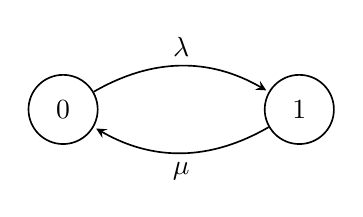
\begin{tikzpicture}[->,>=stealth,shorten >=1pt,auto,node distance=3cm,semithick]
\tikzstyle{every state}=[fill=white,draw=black,text=black,minimum size=25pt]
\node[state] (0) {$0$};
\node[state] (1) [right of=0] {$1$};
\path 
(0) edge[bend left] node[above] {$\lambda$} (1)
(1) edge[bend left] node[below] {$\mu$} (0);
\end{tikzpicture}
\end{center}

\begin{equation*}
\begin{pmatrix}
P'_t(0,0) & P'_t(0,1) \\
P'_t(1,0) & P'_t(1,1)
\end{pmatrix} = \begin{pmatrix}
-\lambda & \lambda \\
\mu & -\mu
\end{pmatrix} \begin{pmatrix}
P_t(0,0) & P_t(0,1) \\
P_t(1,0) & P_t(1,1)
\end{pmatrix}
\end{equation*}

\begin{align*}
P'_t(0,0) &= -\lambda P_t(0,0) + \mu P_t(1,0) \\
P'_t(1,0) &= \lambda P_t(0,0) - \mu P_t(1,0)
\end{align*}

\textbf{Restando}:
\begin{align*}
P'_t(0,0) - P'_t(1,0) &= -(\mu + \lambda) P_t(0,0) + (\mu + \lambda) P_t(1,0) \\
P'_t(0,0) - P'_t(1,0) &= -(\mu + \lambda) \big(P_t(0,0) - P_t(1,0)\big) \\
\big(P_t(0,0) - P_t(1,0)\big)' &= -(\mu + \lambda) \big(P_t(0,0) - P_t(1,0)\big)
\end{align*}

Por lo tanto:
\begin{equation*}
P_t(0,0) - P_t(1,0) = Ce^{-(\mu+\lambda)t}
\end{equation*}

Reemplazando en (1):

\begin{equation*}
P'_t(0,0) = -\lambda e^{-(\mu+\lambda)t}
\end{equation*}

\begin{equation*}
\int_0^t P'_s(0,0) ds = \int_0^t -\lambda e^{-(\mu+\lambda)s} ds
\end{equation*}

\begin{equation*}
P_t(0,0) - P_0(0,0) = \frac{\lambda}{\mu+\lambda} \left(e^{-(\mu+\lambda)s}\right)\Bigg|_0^t
\end{equation*}

\begin{equation*}
\Rightarrow P_t(0,0) = 1 + \frac{\lambda}{\mu+\lambda} \left(e^{-(\mu+\lambda)t} - e^{-(\mu+\lambda)0}\right)
\end{equation*}

\begin{equation*}
= 1 - \frac{\lambda}{\mu+\lambda} \left(1 - e^{-(\mu+\lambda)t}\right)
\end{equation*}

\begin{equation*}
= 1 - \frac{\lambda}{\mu+\lambda} + \frac{\lambda}{\mu+\lambda} e^{-(\mu+\lambda)t}
\end{equation*}

\begin{equation*}
= \frac{\mu}{\mu+\lambda} + \frac{\lambda}{\mu+\lambda} e^{-(\mu+\lambda)t}
\end{equation*}

De manera similar:
\begin{equation*}
P_t(1,0) = \frac{\mu}{\mu+\lambda} - \frac{\mu}{\mu+\lambda} e^{-(\mu+\lambda)t}
\end{equation*}

\begin{equation*}
P_t(0,1) = 1 - P_t(0,0)
\end{equation*}

\begin{equation*}
= \frac{\lambda}{\mu+\lambda} - \frac{\lambda}{\mu+\lambda} e^{-(\mu+\lambda)t}
\end{equation*}

\begin{equation*}
P_t(1,1) = 1 - P_t(1,0)
\end{equation*}

\begin{equation*}
= \frac{\lambda}{\mu+\lambda} + \frac{\mu}{\mu+\lambda} e^{-(\mu+\lambda)t}
\end{equation*}

% ===================== Comportamiento límite =====================

\textbf{Comportamiento límite:}

\definicion{Una cadena de Markov en tiempo continuo es irreducible si para todo $x, y \in S$, existe una secuencia de estados $x_0 = x, x_1, \ldots, x_n = y$ tal que
\begin{equation*}
q(x_{m-1}, x_m) > 0 \quad \text{para } 1 \leq m \leq n.
\end{equation*}}

\begin{center}
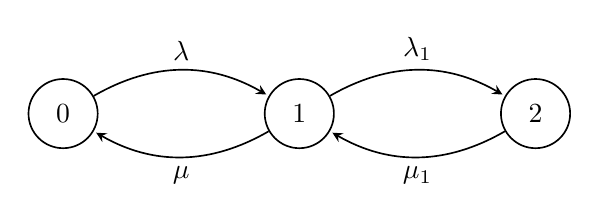
\begin{tikzpicture}[->,>=stealth,shorten >=1pt,auto,node distance=3cm,semithick]
\tikzstyle{every state}=[fill=white,draw=black,text=black,minimum size=25pt]
\node[state] (0) {$0$};
\node[state] (1) [right of=0] {$1$};
\node[state] (2) [right of=1] {$2$};
\path 
(0) edge[bend left] node[above] {$\lambda$} (1)
(1) edge[bend left] node[below] {$\mu$} (0)
(1) edge[bend left] node[above] {$\lambda_1$} (2)
(2) edge[bend left] node[below] {$\mu_1$} (1)
;
\end{tikzpicture}
\end{center}

\definicion{La medida $\pi$ sobre $S$ es estacionaria si
\begin{equation*}
\pi P_t = \pi.
\end{equation*}
}


\teorema{$\pi$ es una medida estacionaria si y solo si
\begin{equation*}
\pi Q = 0.
\end{equation*}
}

\textbf{Demostración}:

\begin{itemize}
\item Si $\pi$ es estacionaria: $\pi P_t = \pi$.
\begin{align*}
\Rightarrow \pi \frac{dP_t}{dt} &= 0 \\
\Rightarrow \pi P_t Q &= 0 \leftarrow \text{Kolmogorov} \\
\Rightarrow \pi Q &= 0 \leftarrow \text{estacionaria}.
\end{align*}
\end{itemize}

Si $\pi P_t = \pi$.

\begin{align*}
\frac{d}{dt} \pi P_t &= \pi \frac{dP_t}{dt} = \pi Q P_t = 0
\end{align*}

$\Rightarrow \pi P_t = \text{constante}$.

cuando $t = 0$, $P_t = \text{id}$.

Luego, constante $= \pi$.

% ===================== Problema: Determinar π cuando se conoce Q =====================

\textbf{Problema}: Determinar $\pi$ cuando

\begin{equation*}
Q = \begin{pmatrix}
-\lambda & \lambda \\
\mu & -\mu
\end{pmatrix}
\end{equation*}

\textbf{Solución:} $\pi Q = 0$

\begin{equation*}
\Rightarrow \quad (\pi_0, \pi_1) \begin{pmatrix}
-\lambda & \lambda \\
\mu & -\mu
\end{pmatrix} = (0, 0)
\end{equation*}

\begin{align*}
\Rightarrow -\lambda \pi_0 + \mu \pi_1 &= 0 \\
\lambda \pi_0 - \mu \pi_1 &= 0 \\
\pi_0 + \pi_1 &= 1
\end{align*}

\begin{equation*}
\Rightarrow \quad \pi = \left(\frac{\mu}{\mu + \lambda}, \frac{\lambda}{\mu + \lambda}\right)
\end{equation*}

De la ecuación:
\begin{align*}
-\lambda \pi_0 + \mu(1-\pi_0) &= 0 \\
-\lambda \pi_0 + \mu - \mu\pi_0 &= 0 \\
\Rightarrow \pi_0 &= \frac{\mu}{\lambda + \mu} \\
\pi_1 &= 1 - \frac{\mu}{\lambda + \mu} = \frac{\lambda}{\lambda + \mu}
\end{align*}

\teorema{Si $(X_t)_{t \geq 0}$ es una cadena de Markov irreducible y recurrente positiva, entonces
\begin{equation*}
P_t(i,j) \to \pi(j).
\end{equation*}

Además: Si $r(i)$ es una recompensa que se gana en el estado $i$ y $\sum_i r(i) \pi(i) < \infty$ entonces
\begin{equation*}
\frac{1}{t} \int_0^t r(X_s) ds \to \sum_j r(j) \pi(j).
\end{equation*}}

% ===================== Problema: Molécula de hemoglobina =====================

\textbf{Problema}: Una molécula de hemoglobina puede transportar una molécula de oxígeno (+) o una molécula de monóxido de carbono (-).

Supongamos que los dos tipos de gases llegan con tasa 1 y 2 y en el tiempo que se conectan con tasas 3 y 4, respectivamente. Considerando el estado 0 cuando la molécula de hemoglobina está libre. Determinar en el largo plazo, la fracción de tiempo que la molécula de hemoglobina está en cada uno de sus tres estados $(-, 0, +)$.

\textbf{Sol:}

\begin{center}
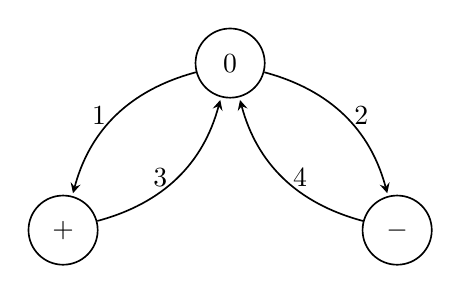
\begin{tikzpicture}[->,>=stealth,shorten >=1pt,auto,node distance=3cm,semithick]
\tikzstyle{every state}=[fill=white,draw=black,text=black,minimum size=25pt]
\node[state] (0) {$0$};
\node[state] (plus) [below left of=0] {$+$};
\node[state] (minus) [below right of=0] {$-$};
\path 
(0) edge[bend right] node[left] {$1$} (plus)
(plus) edge[bend right] node[left] {$3$} (0)
(0) edge[bend left] node[right] {$2$} (minus)
(minus) edge[bend left] node[right] {$4$} (0);
\end{tikzpicture}
\end{center}

\begin{equation*}
Q = \begin{pmatrix}
-3 & 0 & 3 \\
1 & -4 & 4 \\
2 & 0 & -3
\end{pmatrix}
\begin{matrix}
- \\
0 \\
+
\end{matrix}
\end{equation*}

\begin{equation*}
\pi Q = 0
\end{equation*}

\begin{equation*}
(\pi(-), \pi(0), \pi(+)) \begin{pmatrix}
-4 & 4 & 0 \\
2 & -3 & 1 \\
0 & 3 & -3
\end{pmatrix} = (0, 0, 0)
\end{equation*}


\begin{align*}
-4\pi(-) + 2\pi(0) &= 0 \\
4\pi(-) - 3\pi(0) + 3\pi(+) &= 0 \\
\pi(0) - 3\pi(+) &= 0 \\
\pi(-) + \pi(0) + \pi(+) &= 1
\end{align*}

\begin{equation*}
\pi(+) = \frac{2}{11}, \quad \pi(0) = \frac{6}{11}, \quad \pi(-) = \frac{3}{11}
\end{equation*}

% ===================== Procesos de Nacimiento y Muerte =====================

\section*{Procesos de Nacimiento y Muerte}

\definicion{Un proceso de nacimiento y muerte se define por:
\begin{align*}
q(i, i+1) &= \lambda_i \\
q(i, i-1) &= \mu_i
\end{align*}
para todo $i$. $X_t :$ Número de partículas en un sistema en un tiempo $t$.}

\begin{itemize}
\item \textbf{Proceso de nacimiento puro:}
\begin{align*}
q(i, i+1) &= \lambda_i \\
q(i, i-1) &= 0
\end{align*}

\item \textbf{Proceso de Poisson:}
\begin{align*}
q(i, i+1) &= \lambda \\
q(i, i-1) &= 0
\end{align*}

\item \textbf{Proceso de Yule:}

\begin{center}
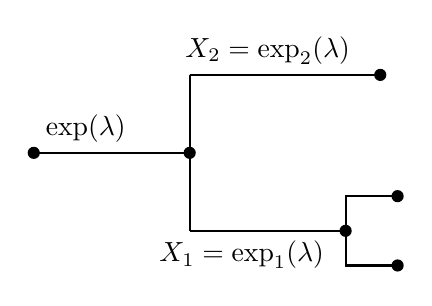
\begin{tikzpicture}[scale=1.1,thick]
% spine
\coordinate (top) at (0,1.2);
\coordinate (mid) at (0,0.3);
\coordinate (bottom) at (0,-0.6);
\draw (top) -- (bottom);

% left branch
\coordinate (left) at (-1.8,0.3);
\draw (mid) -- (left);

% upper branch to the right
\coordinate (topr) at (2.2,1.2);
\draw (top) -- (topr);

% lower branch with small jump
\coordinate (botr1) at (1.8,-0.6);
\coordinate (botr2) at (1.8,-0.2);
\coordinate (botr3) at (2.4,-0.2);
\coordinate (botr4) at (1.8,-1.0);
\coordinate (botr5) at (2.4,-1.0);

\draw (bottom) -- (botr1) -- (botr2) -- (botr3);
\draw (botr2) -- (botr4) -- (botr5);

% points
\fill (mid) circle (2pt);
\fill (left) circle (2pt);
\fill (topr) circle (2pt);
\fill (botr1) circle (2pt);
\fill (botr3) circle (2pt);
\fill (botr5) circle (2pt);

% labels
\node[above] at (-1.2,0.3) {$\exp(\lambda)$};
\node[above] at (0.9,1.2) {$X_2 = \exp_2(\lambda)$};
\node[below] at (0.6,-0.6) {$X_1 = \exp_1(\lambda)$};
\end{tikzpicture}
\end{center}

\begin{align*}
P\left(\min(X_1, X_2) \geq t\right) &= P(X_1 \geq t, X_2 \geq t) \\
&= P(X_1 \geq t) \cdot P(X_2 \geq t) \\
&= e^{-\lambda t} \cdot e^{-\lambda t} = e^{-2\lambda t}
\end{align*}

\begin{align*}
q(i, i+1) &= i\lambda \\
q(i, i-1) &= 0
\end{align*}

\item \textbf{Proceso de Ramificación:}
\begin{align*}
q(i, i+1) &= i\lambda \\
q(i, i-1) &= i\mu
\end{align*}
\end{itemize}

% ===================== Medida Estacionaria de Proceso de Nacimiento y Muerte =====================

Determinemos la medida estacionaria de un proceso de nacimiento y muerte.

\begin{align*}
q(i, i+1) &= \lambda_i \quad ; \quad i = 0, 1, 2, \ldots \\
q(i, i-1) &= \mu_i \quad ; \quad i = 1, 2, \ldots
\end{align*}

\begin{equation*}
Q = \begin{pmatrix}
-\lambda_0 & \lambda_0 & 0 & 0 & 0 & \cdots \\
\mu_1 & -(\mu_1 + \lambda_1) & \lambda_1 & 0 & 0 & \cdots \\
0 & \mu_2 & -(\mu_2 + \lambda_2) & \lambda_2 & 0 & \cdots \\
0 & 0 & \mu_3 & -(\mu_3 + \lambda_3) & \lambda_3 & \cdots \\
0 & 0 & 0 & \mu_4 & -(\mu_4 + \lambda_4) & \cdots \\
\vdots & \vdots & \vdots & \vdots & \vdots & \ddots
\end{pmatrix}
\end{equation*}

% ===================== Solución de la medida estacionaria =====================

$(\pi_0, \pi_1, \pi_2, \ldots) Q = (0, 0, 0, \ldots)$

\begin{align*}
\mu_1 \pi_1 &= \lambda_0 \pi_0 \\
\lambda_0 \pi_0 - (\mu_1 + \lambda_1) \pi_1 + \mu_2 \pi_2 &= 0 \quad \Rightarrow \lambda_1 \pi_1 = \mu_2 \pi_2 = \mu_1 \pi_1 + \lambda_1 \pi_1 \\
\lambda_1 \pi_1 + \mu_3 \pi_3 &= \mu_2 \pi_2 + \lambda_2 \pi_2 \\
\lambda_{n-1} \pi_{n-1} + \mu_{n+1} \pi_{n+1} &= \mu_n \pi_n + \lambda_n \pi_n
\end{align*}

\begin{align*}
\pi_1 &= \frac{\lambda_0}{\mu_1} \pi_0 \\
\Rightarrow \lambda_0 \pi_0 - (\mu_1 + \lambda_1) \frac{\lambda_0}{\mu_1} \pi_0 + \mu_2 \pi_2 &= 0 \\
\lambda_0 \pi_0 - \mu_1 \frac{\lambda_0}{\mu_1} \pi_0 - \lambda_1 \frac{\lambda_0}{\mu_1} \pi_0 + \mu_2 \pi_2 &= 0 \\
\pi_2 &= \frac{\lambda_0 \lambda_1}{\mu_1 \mu_2} \pi_0 \\
\lambda_1 \frac{\lambda_0}{\mu_1} \pi_0 + \mu_3 \pi_3 &= \mu_2 \frac{\lambda_0 \lambda_1}{\mu_1 \mu_2} \pi_0 + \lambda_2 \frac{\lambda_0 \lambda_1}{\mu_1 \mu_2} \pi_0 \\
\pi_3 &= \frac{\lambda_0 \lambda_1 \lambda_2}{\mu_1 \mu_2 \mu_3} \pi_0
\end{align*}

\begin{equation*}
\pi_n = \frac{\lambda_0 \lambda_1 \lambda_2 \cdots \lambda_{n-1}}{\mu_1 \mu_2 \mu_3 \cdots \mu_n} \pi(0)
\end{equation*}

\begin{align*}
\sum_{n=0}^{\infty} \pi(n) &= 1 \\
\pi(0) + \pi(1) + \pi(2) + \cdots + \pi(n) + \cdots &= 1 \\
\pi(0) + \frac{\lambda_0}{\mu_1} \pi(0) + \frac{\lambda_0 \lambda_1}{\mu_1 \mu_2} \pi(0) + \cdots + \frac{\lambda_0 \lambda_1 \cdots \lambda_{n-1}}{\mu_1 \mu_2 \cdots \mu_n} \pi(0) + \cdots &= 1
\end{align*}

\begin{equation*}
\Rightarrow \left(1 + \sum_{n=1}^{\infty} \frac{\lambda_0 \lambda_1 \cdots \lambda_{n-1}}{\mu_1 \mu_2 \cdots \mu_n}\right) \pi(0) = 1
\end{equation*}

\begin{equation*}
\pi(0) = \left(1 + \sum_{n=1}^{\infty} \frac{\lambda_0 \lambda_1 \cdots \lambda_{n-1}}{\mu_1 \mu_2 \cdots \mu_n}\right)^{-1}
\end{equation*}

% ===================== Diagrama de cadena de nacimiento y muerte =====================

\begin{center}
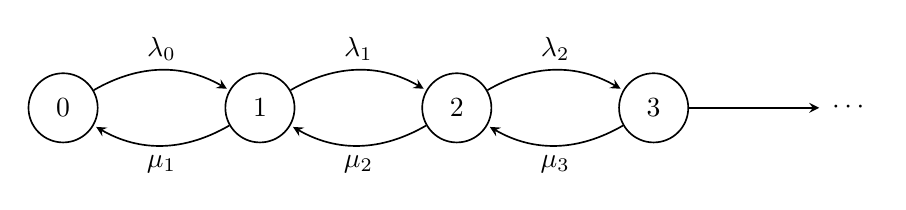
\begin{tikzpicture}[->,>=stealth,shorten >=1pt,auto,node distance=2.5cm,semithick]
\tikzstyle{every state}=[fill=white,draw=black,text=black,minimum size=25pt]

\node[state] (0) {$0$};
\node[state] (1) [right of=0] {$1$};
\node[state] (2) [right of=1] {$2$};
\node[state] (3) [right of=2] {$3$};
\node[right of=3] (dots) {$\cdots$};

\path 
(0) edge[bend left] node[above] {$\lambda_0$} (1)
(1) edge[bend left] node[below] {$\mu_1$} (0)
(1) edge[bend left] node[above] {$\lambda_1$} (2)
(2) edge[bend left] node[below] {$\mu_2$} (1)
(2) edge[bend left] node[above] {$\lambda_2$} (3)
(3) edge[bend left] node[below] {$\mu_3$} (2)
(3) edge node[above] {} (dots);
\end{tikzpicture}
\end{center}

\textbf{Observación}: En proceso de nacimiento y muerte existe la medida estacionaria si
\begin{equation*}
\sum_{n=1}^{\infty} \frac{\lambda_0 \lambda_1 \cdots \lambda_{n-1}}{\mu_1 \mu_2 \cdots \mu_n} < \infty.
\end{equation*}

\end{document}
